\chapter{Context engineering and repository comprehension}

\section{Engineering principles}

Context is a scarce working set, not a database. Start from repository purpose and an architecture map, then trace a concrete behavior from entry point through domain logic, persistence and tests. Search for definitions, callers and configuration edges rather than reading files alphabetically. Preserve provenance with commit SHA and path; summaries may omit invariants or become stale after a branch change.\src{O7,A2,A9}

\section{Implementation approach}

Create a context manifest listing the task, architecture boundaries, relevant symbols, source paths and unresolved questions. Retrieve only the evidence needed for the current decision. Summarize confirmed facts separately from hypotheses. When compacting, retain test failures, decisions, prohibited actions and next steps. At resume, compare the baseline SHA and re-read changed files. Keep independent workstreams in separate contexts.

\section{Verification and limitations}

Validate a comprehension report by tracing one end-to-end path and locating a test for each important invariant. Never inject entire issue comments or tool results as trusted instructions. Persistent memory changes should be reviewed and should not include credentials.

Figure~\ref{fig:d7} illustrates the conceptual flow from Task contract to Agent session. The edges describe the proposed integration or control relationship, not undocumented internal calls.

\begin{figure}[htbp]\centering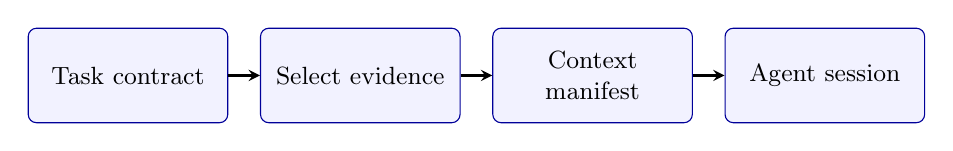
\begin{tikzpicture}[nodebox/.style={draw=blue!60!black,fill=blue!5,rounded corners=3pt,minimum height=12mm,text width=23mm,align=center,font=\small},>=stealth]
\node[nodebox] (n0) at (0.00,0.00) {Task contract};
\node[nodebox] (n1) at (2.95,0.00) {Select evidence};
\node[nodebox] (n2) at (5.90,0.00) {Context manifest};
\node[nodebox] (n3) at (8.85,0.00) {Agent session};
\draw[->,thick] (n0.east) -- (n1.west);
\draw[->,thick] (n1.east) -- (n2.west);
\draw[->,thick] (n2.east) -- (n3.west);
\end{tikzpicture}
\caption{Context assembly (conceptual view).}\label{fig:d7}\end{figure}

\section{Chapter conclusion}

Apply the stated verification criteria before expanding the scope of this workflow. Record deviations, evidence and unresolved risks in the task record.
